\documentclass[10pt]{article}
\usepackage[
  paperheight=8.5in, 
  paperwidth=5.5in,
  margin=.4in
]{geometry}
\usepackage[per-mode=symbol]{siunitx}
\usepackage{enumitem,multicol,pgfplots}
\pgfplotsset{
  compat=1.18,
  width=6cm,
  height=7cm,
  posgraph/.append style={
    axis y line = left,
    axis x line = center,
    axis line style = ultra thick,
    xlabel={\bf time},
    ylabel={\bf displacement},
    ymin=0,
    ymax=9,
    xmin=0,
    xmax=3,
    xtick=\empty,
    ytick=\empty,
  },
  velgraph/.append style={
    xlabel={\bf time},
    ylabel={\bf velocity},
    ymin=-5,
    ymax=5,
    xmin=0,
    xmax=4,
    ytick=\empty,
    xtick=\empty,
    axis y line = left,
    axis x line = center,
    axis line style = ultra thick,
  },
  numberedplots/.append style={
    xlabel={\bf time (s)},
    width=7cm,
    ytick={-15,...,15},
    xtick={0,...,5},
    axis y line = left,
    axis x line = center,
    grid=major,
    axis line style = ultra thick,
  },
}


\begin{document}
\pagestyle{empty}

\noindent Consider a graph of an object moving forward and slowing down.

\begin{multicols}{2}

  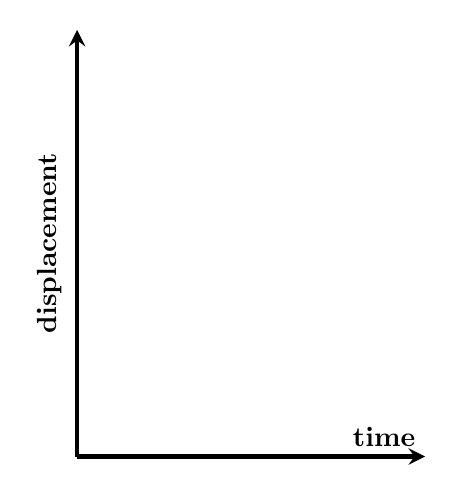
\begin{tikzpicture}
    \begin{axis}[posgraph]
    \end{axis}
  \end{tikzpicture}

  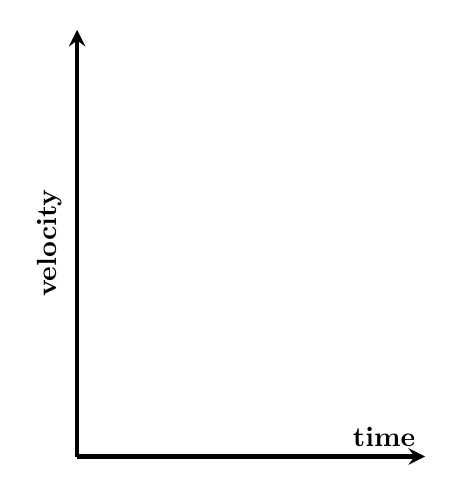
\begin{tikzpicture}
    \begin{axis}[
      posgraph,
      ylabel={\bf velocity}
    ]
    \end{axis}
  \end{tikzpicture}
  
\end{multicols}

What we can learn from graphs:

\begin{multicols}{2}
  {\bf Displacement Graphs}

  \vspace{3em}

  slope = 

  \vspace{5em}

  moving forward:

  \vspace{2em}
  
  moving backward:


  \vspace{7em}

  fast:

  \vspace{2em}
  
  slow:



  \columnbreak

  {\bf Velocity Graphs}

  \vspace{3em}

  slope = 

  \vspace{5em}

  moving forward:

  \vspace{2em}
  
  moving backward:


  \vspace{7em}

  fast:

  \vspace{2em}
  
  slow:


  
\end{multicols}


\end{document}